\section{Advanced data analytics}

Advanced analytics encompasses a range of sophisticated data analysis methods that are pivotal in the business context. 
These techniques span varying levels of complexity and value, categorized into four primary types: descriptive, diagnostic, predictive, and prescriptive analytics.
The overarching goal is to uncover hidden patterns, predict future trends, and facilitate data-driven decision-making.

\begin{definition}[\textit{Data}]
    Data are raw, unprocessed facts that serve as the basic unit of measurable information.
\end{definition}
\begin{definition}[\textit{Information}]
    Information is processed and organized data that becomes meaningful and useful.
\end{definition}
\begin{definition}[\textit{Knowledge}]
    Knowledge arises when information is combined with experience, expertise, and authoritative judgment, leading to actionable decisions.
\end{definition}

\begin{figure}[H]
    \centering
    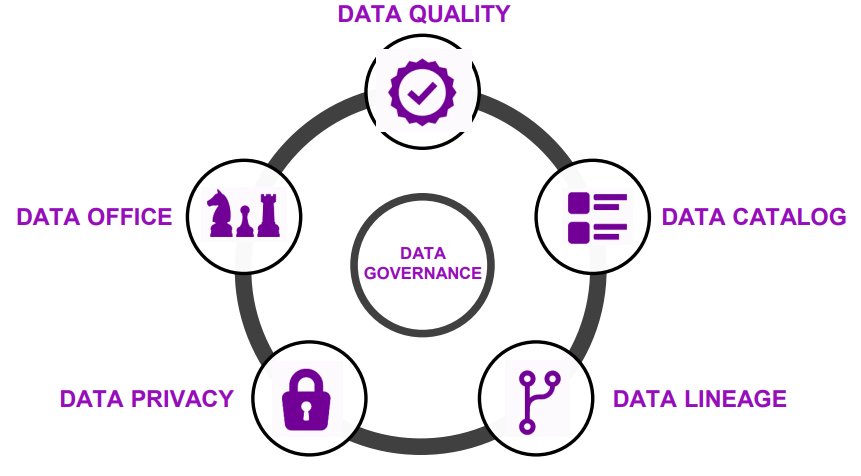
\includegraphics[width=0.5\linewidth]{images/bis5.png}
    \caption{Data analytics levels}
\end{figure}

\subsection{Business intelligence}
Business Intelligence (BI) refers to a set of methodologies, processes, architectures, and technologies that transform raw data into meaningful and actionable information. 
BI enables more effective strategic, tactical, and operational decision-making.

BI primarily focuses on historical reporting, utilizing descriptive and diagnostic analytics to help organizations understand past performance.
Advanced analytics builds upon this foundation by incorporating predictive and prescriptive capabilities, enabling deeper insights into future trends and optimal actions.

\paragraph*{Design}
A BI system is typically designed through the following steps:
\begin{enumerate}
    \item \textit{Data identification and structuring}: identifying relevant data and organizing it into a usable format.
    \item \textit{Expected output definition}: defining the expected results and objectives of the analysis.
    \item \textit{Database model and design}: creating appropriate data structures to store and manage the data.
    \item \textit{Dashboards and visual design}: developing user-friendly dashboards and visualizations to present data meaningfully.
\end{enumerate}

\begin{figure}[H]
    \centering
    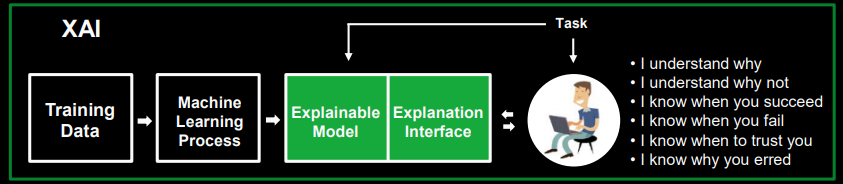
\includegraphics[width=0.5\linewidth]{images/bis6.png}
    \caption{Business intelligence architecture}
\end{figure}

\paragraph*{Levels}
BI systems cater to three primary user groups:
\begin{enumerate}
    \item \textit{Technical BI} (IT end users): focuses on the infrastructure and backend of BI systems.
    \item \textit{Self-service BI} (analysts): enables business analysts to explore data and generate insights independently.
    \item \textit{End-user BI} (everyone): designed for general users across the organization to access insights and make data-driven decisions.
\end{enumerate}
\noindent To transform raw data into actionable knowledge and tangible value, the following considerations are essential: quality of data, context, business relevance, and agility

\begin{figure}[H]
    \centering
    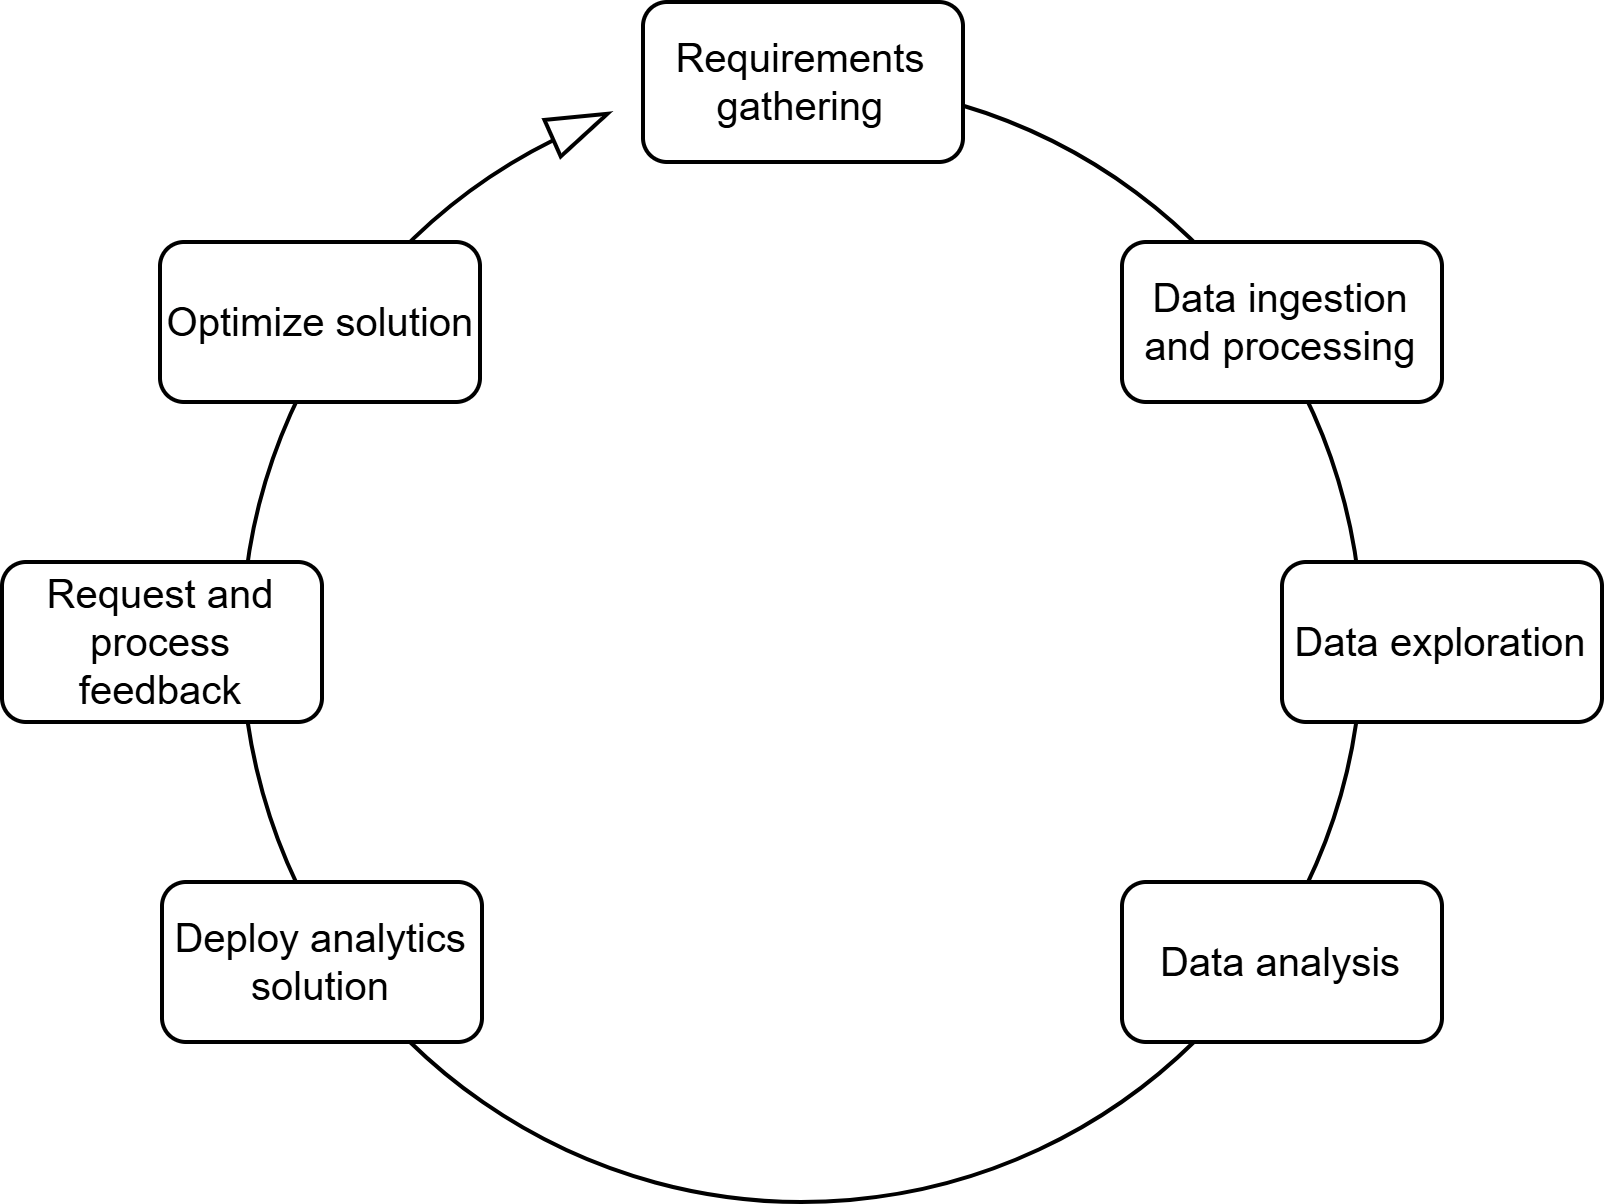
\includegraphics[width=0.5\linewidth]{images/bis7.png}
    \caption{Business information lifecycle}
\end{figure}

\subsection{Power BI}
Power BI Desktop is a free tool that empowers users to create rich, interactive reports with visual analytics from hundreds of data sources. 
Its development methodology follows these key steps:
\begin{enumerate}
    \item \textit{Query creation}: filtering, formatting, and refining data to ensure accuracy and relevance.
    \item \textit{Relationship configuration}: establishing the foundations of a data model by defining relationships between datasets.
    \item \textit{Data model enrichment}: adding calculation logic, measures, and formatting to enhance the data model.
    \item \textit{Data exploration}: using drag-and-drop functionality on the Canvas to explore data in innovative ways.
    \item \textit{Interactive report design}: creating reports with a wide range of customizable data visualizations.
    \item \textit{Publishing}: sharing and consuming the report content online for broader accessibility and collaboration.
\end{enumerate}
